\documentclass[spec, och, labwork]{shiza}
% параметр - тип обучения - одно из значений:
%    spec     - специальность
%    bachelor - бакалавриат (по умолчанию)
%    master   - магистратура
% параметр - форма обучения - одно из значений:
%    och   - очное (по умолчанию)
%    zaoch - заочное
% параметр - тип работы - одно из значений:
%    referat    - реферат
%    coursework - курсовая работа (по умолчанию)
%    diploma    - дипломная работа
%    pract      - отчет по практике
% параметр - включение шрифта
%    times    - включение шрифта Times New Roman (если установлен)
%               по умолчанию выключен
\usepackage{subfigure}
\usepackage{tikz,pgfplots}
\pgfplotsset{compat=1.5}
\usepackage{float}

%\usepackage{titlesec}
\setcounter{secnumdepth}{4}
%\titleformat{\paragraph}
%{\normalfont\normalsize}{\theparagraph}{1em}{}
%\titlespacing*{\paragraph}
%{35.5pt}{3.25ex plus 1ex minus .2ex}{1.5ex plus .2ex}

\titleformat{\paragraph}[block]
{\hspace{1.25cm}\normalfont}
{\theparagraph}{1ex}{}
\titlespacing{\paragraph}
{0cm}{2ex plus 1ex minus .2ex}{.4ex plus.2ex}

% --------------------------------------------------------------------------%


\usepackage[T2A]{fontenc}
\usepackage[utf8]{inputenc}
\usepackage{graphicx}
\graphicspath{ {./images/} }
\usepackage{tempora}

\usepackage[sort,compress]{cite}
\usepackage{amsmath}
\usepackage{amssymb}
\usepackage{amsthm}
\usepackage{fancyvrb}
\usepackage{listings}
\usepackage{listingsutf8}
\usepackage{longtable}
\usepackage{array}
\usepackage[english,russian]{babel}

% \usepackage[colorlinks=true]{hyperref}
\usepackage{url}

\usepackage{underscore}
\usepackage{setspace}
\usepackage{indentfirst} 
\usepackage{mathtools}
\usepackage{amsfonts}
\usepackage{enumitem}
\usepackage{tikz}
\usepackage{minted}

\newcommand{\eqdef}{\stackrel {\rm def}{=}}
\newcommand{\specialcell}[2][c]{%
\begin{tabular}[#1]{@{}c@{}}#2\end{tabular}}

\renewcommand\theFancyVerbLine{\small\arabic{FancyVerbLine}}

\newtheorem{lem}{Лемма}

\begin{document}

% Кафедра (в родительном падеже)
\chair{}

% Тема работы
\title{Логические элементы и схемы}

% Курс
\course{3}

% Группа
\group{331}

% Факультет (в родительном падеже) (по умолчанию "факультета КНиИТ")
\department{факультета КНиИТ}

% Специальность/направление код - наименование
%\napravlenie{09.03.04 "--- Программная инженерия}
%\napravlenie{010500 "--- Математическое обеспечение и администрирование информационных систем}
%\napravlenie{230100 "--- Информатика и вычислительная техника}
%\napravlenie{231000 "--- Программная инженерия}
\napravlenie{100501 "--- Компьютерная безопасность}

% Для студентки. Для работы студента следующая команда не нужна.
% \studenttitle{Студентки}

% Фамилия, имя, отчество в родительном падеже
\author{Стаина Романа Игоревича и Токарева Никиты Сергеевича}

% Заведующий кафедрой
% \chtitle{} % степень, звание
% \chname{}

%Научный руководитель (для реферата преподаватель проверяющий работу)
\satitle{аспирант} %должность, степень, звание
\saname{А. А. Мартышкин}

% Руководитель практики от организации (только для практики,
% для остальных типов работ не используется)
% \patitle{к.ф.-м.н.}
% \paname{С.~В.~Миронов}

% Семестр (только для практики, для остальных
% типов работ не используется)
%\term{8}

% Наименование практики (только для практики, для остальных
% типов работ не используется)
%\practtype{преддипломная}

% Продолжительность практики (количество недель) (только для практики,
% для остальных типов работ не используется)
%\duration{4}

% Даты начала и окончания практики (только для практики, для остальных
% типов работ не используется)
%\practStart{30.04.2019}
%\practFinish{27.05.2019}

% Год выполнения отчета
\date{2022}

\maketitle

% Включение нумерации рисунков, формул и таблиц по разделам
% (по умолчанию - нумерация сквозная)
% (допускается оба вида нумерации)
% \secNumbering

%-------------------------------------------------------------------------------------------
\section{Цель работы:}

Ознакомление с основными характеристиками и испытание интегральных триггеров RS, D, T и JK.

\textbf{Задание 1.}

Построим схему асинхронного RS-триггера.

\begin{figure}[H]
    \centering
    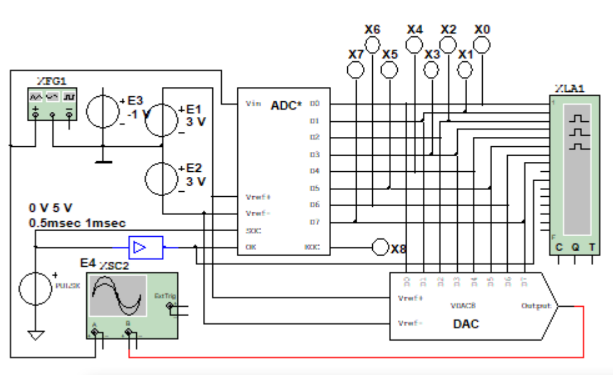
\includegraphics[width=0.7\textwidth]{img/image1}
    \caption{Асинхронный RS-триггер}
\end{figure}
        
Воспользуемся порядком засвечивания разноцветных пробников и зададим коды (00, 01, 10), состояния ключей 1 и 2 (входных сигналов). Наблюдаем:

Код 11

\begin{figure}[H]
    \centering
    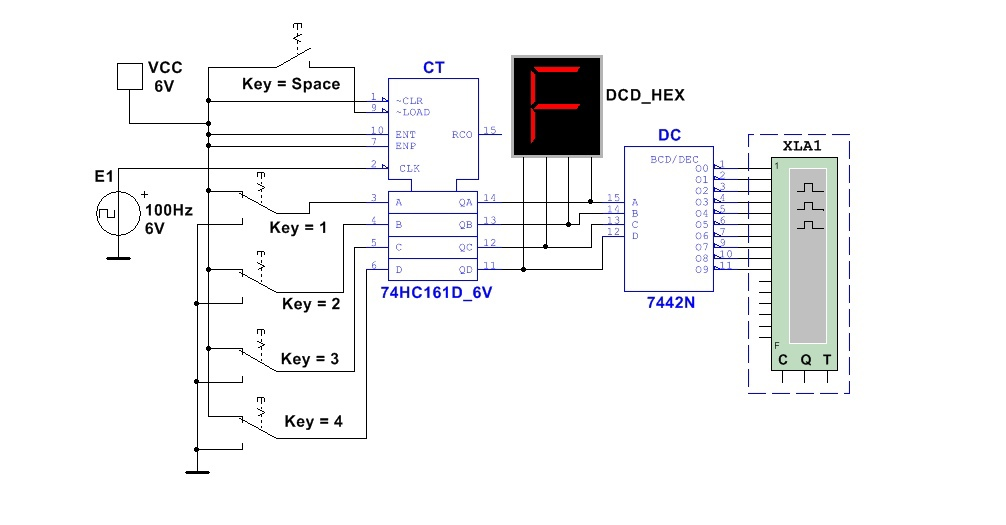
\includegraphics[width=0.7\textwidth]{img/image2}
    \caption{}
\end{figure}

\begin{figure}[H]
    \centering
    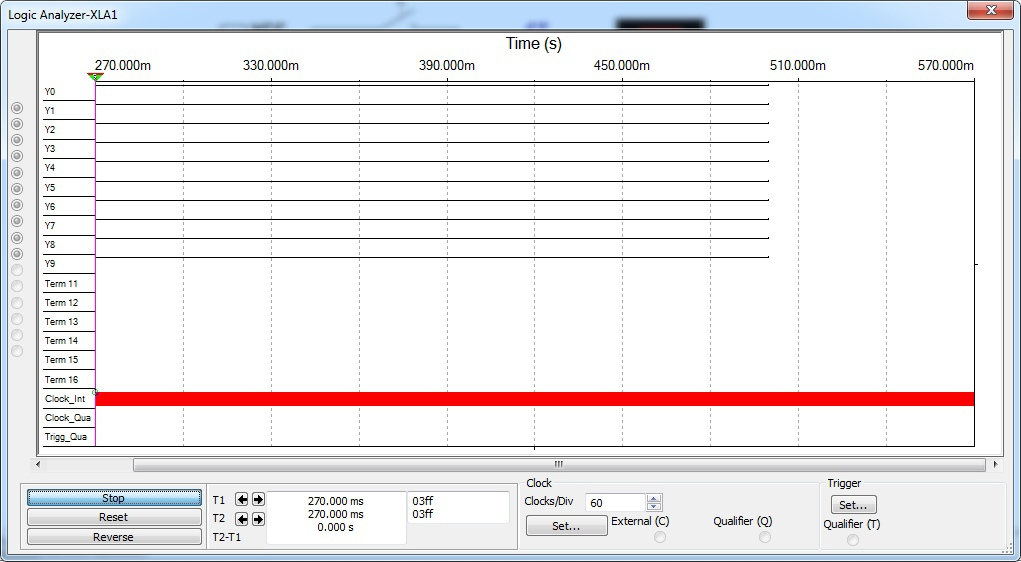
\includegraphics[width=0.7\textwidth]{img/image3}
    \caption{}
\end{figure}

Код 10

\begin{figure}[H]
    \centering
    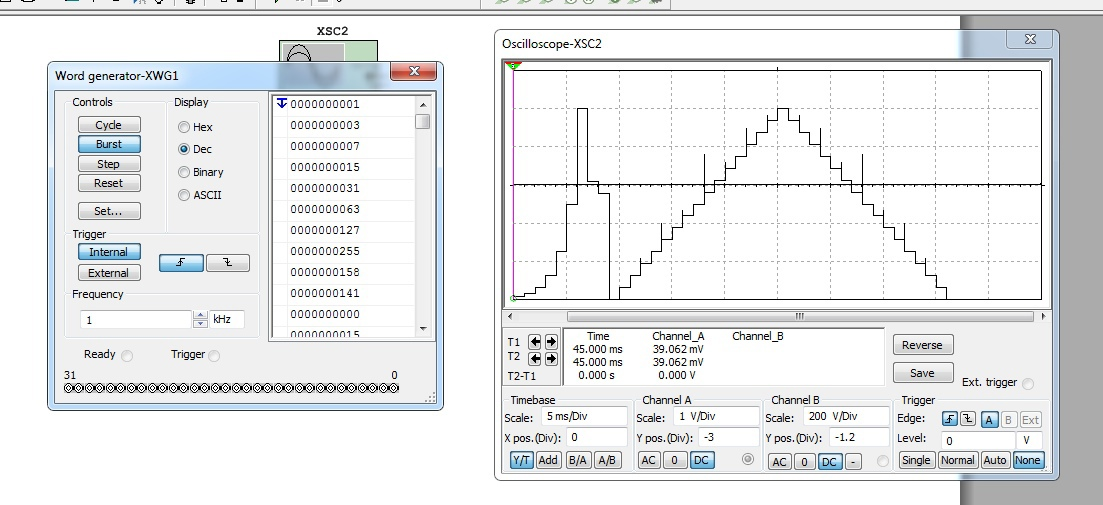
\includegraphics[width=0.7\textwidth]{img/image4}
    \caption{}
\end{figure}

\begin{figure}[H]
    \centering
    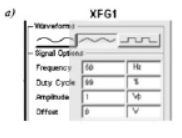
\includegraphics[width=0.7\textwidth]{img/image5}
    \caption{}
\end{figure}

Код 00

\begin{figure}[H]
    \centering
    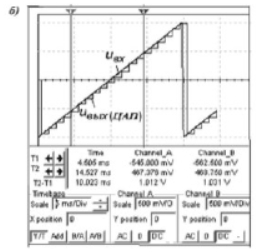
\includegraphics[width=0.7\textwidth]{img/image6}
    \caption{}
\end{figure}

Код 01

\begin{figure}[H]
    \centering
    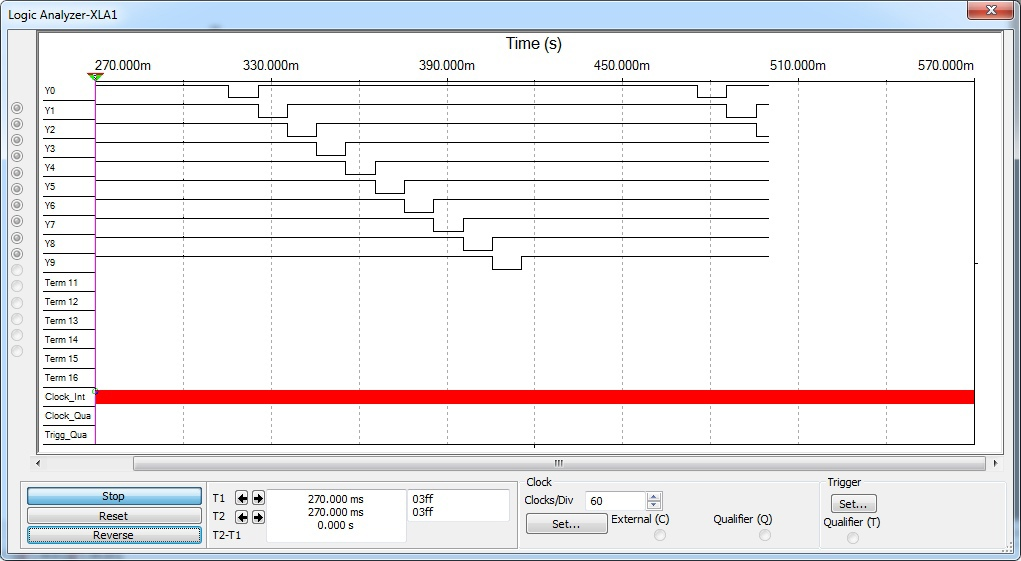
\includegraphics[width=0.7\textwidth]{img/image7}
    \caption{}
\end{figure}

\begin{figure}[H]
    \centering
    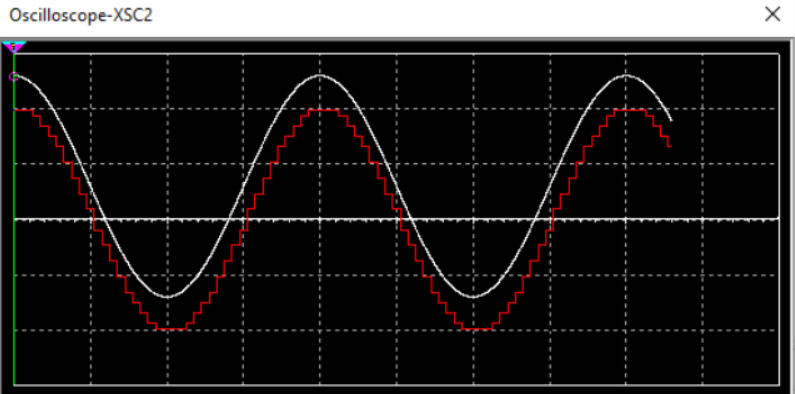
\includegraphics[width=0.7\textwidth]{img/image8}
    \caption{}
\end{figure}

По этим наблюдениям составим таблицу иcтинности RS-триггера.

\begin{table}[H]
    \caption{}
    \label{tabular:timesandtenses}
    \begin{center}
    \begin{tabular}{|c|c|c|c|}
        \hline
    S & R & Q & -Q  \\ \hline
    0 & 0 & 1 & 0 \\ \hline
    0 & 1 & 0 & 1 \\ \hline
    1 & 0 & 1 & 0   \\ \hline
    \end{tabular}
    \end{center}
\end{table}

\textbf{Задание 2.}

Подключим ко входам триггера логический генератор (генератор слова) XWG1, запрограммировав его первые три ячейки кодами 00, 10 и 01 и соединив входы и выходы триггера с входами логического анализатора XLA2. Зададим частоту генератора f =10 кГц и два цикла моделирования сигналов, а в окне анализатора зададим частоту f = 0.1 МГц таймера, уровень высокого напряжения равный U = 5 В и число импульсов, равное 8 таймерам, приходящихся на одно деление. 

\begin{figure}[H]
    \centering
    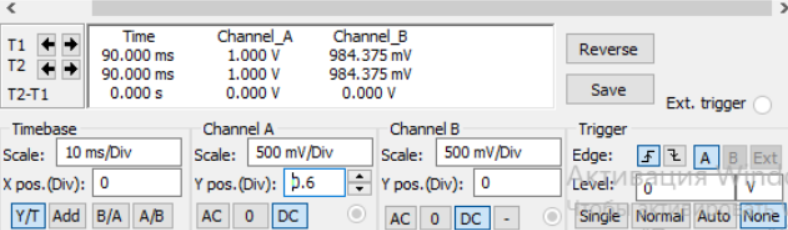
\includegraphics[width=0.7\textwidth]{img/image9}
    \caption{}
\end{figure}

\textbf{Задание 3.} Соберем схему для испытания триггеров JK, T и D. Установим в диалоговых окнах компонентов их параметры или режимы работы.

\begin{figure}[H]
    \centering
    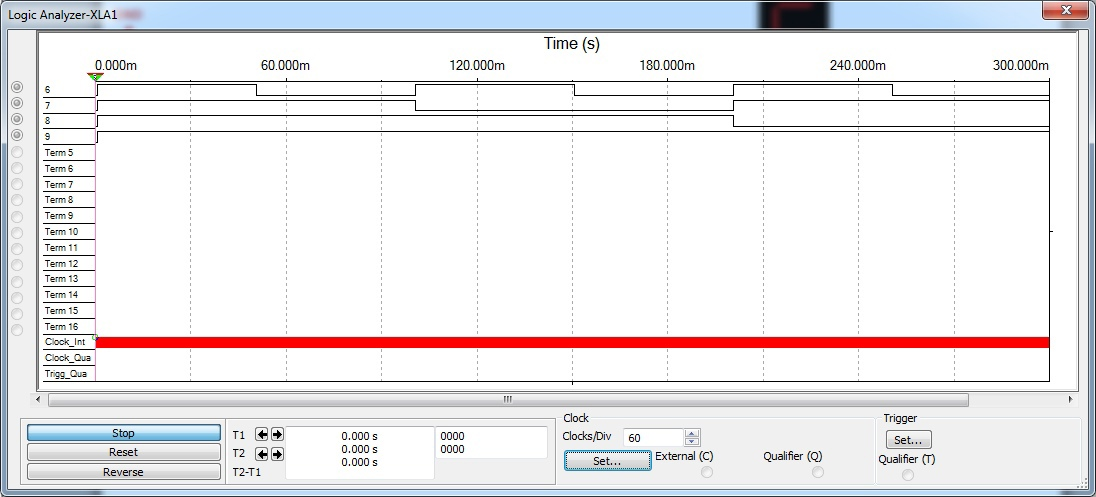
\includegraphics[width=0.7\textwidth]{img/image10}
    \caption{}
\end{figure}

Для формирования выходных сигналов генератор нужно запрограммировать, то есть ввести в ячейки памяти кодовые комбинации из единиц и нулей согласно варианту 1: 0000 1010 1111 1001 1001 1101 1100 0000. Получим:

\begin{figure}[H]
    \centering
    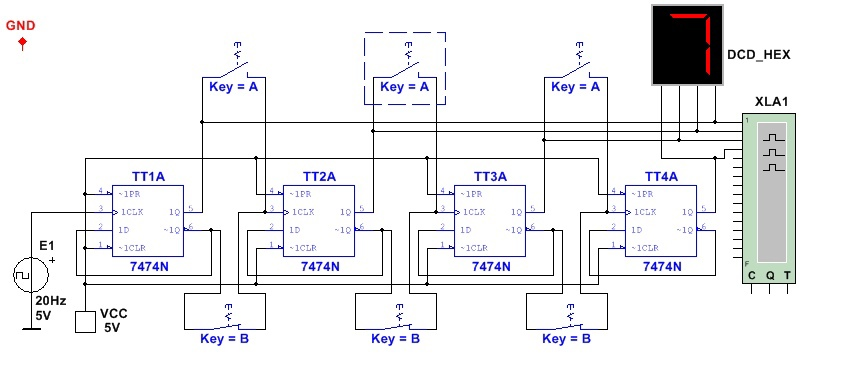
\includegraphics[width=0.85\textwidth]{img/image11}
    \caption{}
\end{figure}

\begin{figure}[H]
    \centering
    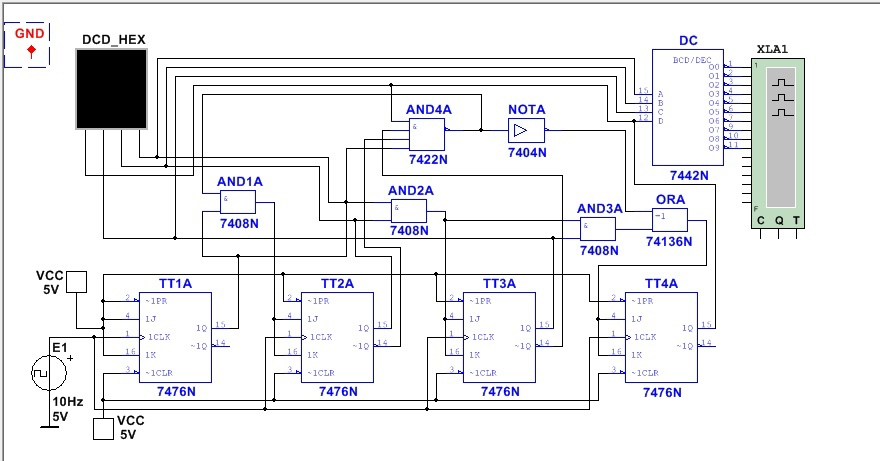
\includegraphics[width=0.7\textwidth]{img/image12}
    \caption{}
\end{figure}

\textbf{Вывод:} ознакомились с основными характеристиками и испытали интегральные триггеры RS, D, T и JK.

\section{Тестовые задания к работе 32:}

\begin{enumerate}
    \item Укажите, какая комбинация логических сигналов является запрещённой для асинхронного RS-триггера:
    
        Ответ: 11.

    \item Укажите условное графическое обозначение:
        
        \begin{itemize}
            \item JK-триггера: г;
            \item RS-триггера: в.
        \end{itemize}
    
        \begin{figure}[H]
            \centering
            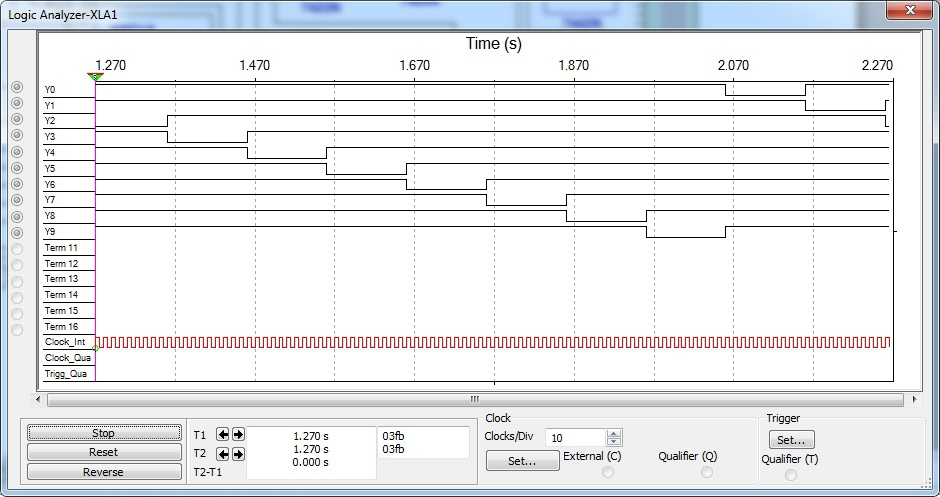
\includegraphics[width=0.7\textwidth]{img/image13}
            \caption{}
        \end{figure}

    \item Укажите условное графическое обозначение:
    
        \begin{itemize}
            \item T-триггера, выполненного на основе JK-триггера: в;
            \item D-триггера, выполненного на основе JK-триггера: д.
        \end{itemize}

        \begin{figure}[H]
            \centering
            \includegraphics[width=0.7\textwidth]{img/image14}
            \caption{}
        \end{figure}

    \item Укажите, как функционирует JK-триггер при комбинации $J = 1, K = 1$ на входе:
    
        Ответ: триггер работает в счётном режиме.

    \item Укажите, нашли ли широкое применение асинхронные D-триггеры:
    
        Ответ: да.
    
    \item Укажите время запаздывания выходного сигнала по отношению к моменту подачи на C-вход D-триггера
    синхроимпульса при тактовой частоте f = 10 кГц ($D^t = 1, Q^t = 0$):

        Ответ: 0.1 мс.
    
    \item Укажите значение сигнала на выходе JK-триггера при комбинации $J = 1, K = 0$ на входе и $Q = 1$ после окончания действия синхроимпульса:

        Ответ: 1.
    
    \item Укажите аналитическое выражение, описывающее работу:
        
        \begin{itemize}
            \item RS-триггера: $Q^{t+1} = S + Q^t \overline{R}$;
            \item JK-триггера: $Q^{t+1} = \overline{K^t} Q^t + J^t \overline{Q^t}$;
            \item T-триггера: $Q^{t+1} = Q^t \overline{T} + \overline{Q^t} T$;
            \item D-триггера: $Q^{t+1} = \overline{C^t} Q^t + C^t Q^t$.
        \end{itemize}
    
    \item Укажите, чем отличается динамическое управление триггерами от статического управления:
    
        Ответ: у триггеров с динамическим управлением сигналы на информационных входах должны оставаться неизменными на всем интервале действия активоного сигнала синхронизации ($C = 1$).
    
    \item Укажите уровни напряжения интегральных микросхем триггеров серии ТТЛ, принимаемые за логическую 1 и логический 0 при напрядении питания $U_n = $ 5 В:

        Ответ: 2,4 В < $U^1$ < 5 В; 0 < $U^0$ < 0.4 В.

    \item Укажите, к какому типу триггеров относят T-триггеры:

        Ответ: к синхронным.

\end{enumerate}

\end{document}
